\documentclass[twocolumn]{iopjournal}

\usepackage{amsmath,amssymb,amsfonts}

\fancyhfoffset[L]{0mm}
\setlength{\marginparwidth}{0pt}
\setlength{\marginparsep}{0pt}

% ==========================================
% ZENODO PREPRINT HEADERS (ACTIVE)
% ==========================================
\renewcommand{\articletype}[1]{%
  {\vspace*{-8mm}\noindent \Large \sf Preprint}\par
  \vspace*{6mm}\noindent{\scriptsize \sf{\bfseries \MakeUppercase{#1}}}}

\fancyhead[L]{}
\fancyhead[R]{}

% ==========================================
% CQG SUBMISSION HEADERS (COMMENTED OUT)
% ==========================================
% \fancyhead[L]{{\small \sf IOP Publishing}\hspace{5mm} {\it Class. Quantum Grav.}}
% \fancyhead[R]{S Nelson}

\begin{document}

\articletype{Letter}

\title{Gravity Field Dynamics: Complete Field Closure from Stellated Octahedron Topology}

\author{Stephen Nelson}

\affil{Field Dynamics Research}

\begin{abstract}
Every formulation of gravity rests on two elements: a topology (the geometric structure of the field) and a closure condition (the requirement that the field extend completely through space). In general relativity, these are the Riemannian manifold and the Einstein field equations; in tetrad gravity, the tetrahedron (vierbein) and metric compatibility; in bimetric gravity, two coupled tetrahedra and ghost-freedom. The tetrahedron appears as the fundamental local frame across each of these formalisms. In every prior case, both the topology and the closure condition are inputs.

We show that both follow from a single equation in combinatorics, $2(d+1) = 2^d$, whose only positive integer solution is $d = 3$. This fixes two structural constants: $K = 4$ vertices per simplex and $D = 3$ spatial dimensions. Binary parity in three dimensions produces two interlocking tetrahedra inscribed in the cube (the stellated octahedron), whose face classification yields the $(3+1)$ spacetime decomposition and whose face normals define the tetrahedron that general relativity abstracts as the tetrad, postulated since Einstein (1928).

The requirement that the field close through this geometry determines the coupling polynomial $f(k,s) = 1 + ks + k^2$, the gravitational constitutive law $\mu(x) = x/(x+1)$, and the complete covariant scalar-tensor action, all with zero free parameters. In bimetric language, the closure geometry fixes the five previously free Hassan--Rosen coefficients to $\{1, 0, 16, 0, 1\}$ (companion letter). The base-8 expansion of pi is algebraically isomorphic to this topology, with structural constants that match the vertex count, channel count, and face count of the stellated octahedron exactly. Every numerical constant in the theory reduces to $K = 4$ and $D = 3$.
\end{abstract}

% ======================================================================
\section*{Introduction}
% ======================================================================

Gravity Field Dynamics (GFD) is a covariant formalism that derives gravitational coupling laws from the discrete combinatorial geometry of the local tetrahedral frame. Like other tetrad formalisms, it operates with dual tetrahedral field chambers. What distinguishes it is that both the topology and the field closure condition are outputs, not inputs.

Every formulation of gravity, from Einstein's metric tensor to Hassan--Rosen bimetric theory, implicitly contains two elements:
\begin{enumerate}
\item A \emph{topology}: the structure of the gravitational field (what the field IS).
\item A \emph{field closure condition}: the requirement that the field must extend completely through space (what the field DOES).
\end{enumerate}

In general relativity, the topology is the Riemannian manifold and the closure condition is that Einstein's equations hold at every spacetime point. In tetrad gravity, the topology is the tetrahedron defined by the vierbein and closure is the metric-compatible connection condition. In bimetric gravity, the topology is two coupled tetrahedra and closure is ghost-freedom; without it, the field cannot close consistently. In scalar-tensor theories, the topology is the scalar field configuration and closure is the constitutive law that governs the interpolation between gravitational regimes.

In each case, both the topology and the closure condition are supplied as starting points. They are inputs to the framework, not results derived from it.

This letter demonstrates that both follow from a single equation in combinatorics:
\begin{equation}
2(d+1) = 2^d.
\end{equation}
The first four sections establish the topology (what the gravitational field IS): the uniqueness theorem forces $d = 3$, binary parity produces the stellated octahedron, face classification yields the $(3+1)$ spacetime decomposition, and the face normals recover the tetrahedron that general relativity abstracts as the tetrad. The remaining sections establish what field closure determines: the coupling constants, the constitutive law, and the complete covariant action, all with zero free parameters.

A companion letter, \emph{Gravity Field Dynamics and Bimetric Gravity: Dual Tetrahedral Field Chambers as the Key to the General Parameters} (Nelson 2026, submitted to \emph{Classical and Quantum Gravity})~\cite{Nelson2026b}, provides the full coupling derivation and ghost-freedom proof. The present letter places those results within the larger chain from combinatorial identity to covariant action. The computational companion \texttt{run\_all\_validations.py} independently verifies every claim.

\subsection{Geometric heritage}

The tetrahedron is the fundamental geometric unit of the local gravitational frame across every major formalism that examines the discrete or interior structure of spacetime. Table~\ref{tab:heritage} summarizes the role it plays in each.

\begin{table}[h]
\centering
\caption{The tetrahedron across gravity formalisms.}
\label{tab:heritage}
{\small
\begin{tabular*}{\columnwidth}{@{\extracolsep{\fill}}lll@{}}
\hline
Formalism & Structure & Geometry \\
\hline
Simplicial (Regge) & 4-simplex & Tetrahedron \\
Tetrad (Cartan/Weyl) & Vierbein & Tet.\ basis \\
LQG / Spin Foams & Spin network & Quantum tet. \\
Bimetric (H-R) & Two tetrads & Two tetrahedra \\
GFD & Dual chambers & Stell.\ oct. \\
\hline
\end{tabular*}}
\end{table}

In textbook simplicial gravity~\cite{Regge1961}, spacetime is triangulated into 4-simplices whose 3-dimensional boundaries are tetrahedra: the discrete volumetric building blocks of curved spacetime.

In textbook tetrad gravity~\cite{Einstein1928,Weyl1929}, the vierbein consists of four linearly independent basis vectors at each spacetime point. Four non-coplanar vectors from a common origin define a tetrahedron. The continuum formalism abstracts this geometry into algebraic vectors, but the underlying object is the tetrahedron.

In loop quantum gravity and spin foam models~\cite{RovelliSmolin1995}, the quantum of three-dimensional space is explicitly defined as a quantum tetrahedron: a spin network node dual to a tetrahedral cell.

In bimetric gravity~\cite{HassanRosen2012a}, two tetrahedra (two tetrads) interact through a potential governed by five free coupling coefficients. The geometric content of that interaction, the face structure of two interlocking tetrahedra, has not previously been evaluated.

GFD evaluates it. The result is the stellated octahedron, and the five coupling coefficients are no longer free.

\subsection{Interior field dynamics}

In general relativity, the Israel junction conditions~\cite{Israel1966} require a structured hypersurface wherever two distinct metric regions meet. An analogous situation arises at the local frame level in bimetric gravity: two tetrahedra share the same tangent space at the field origin, and their interaction cannot be unstructured. The interpenetration of two tetrahedral volumes produces a discrete interior boundary with a definite face geometry, much as two soap bubbles of different pressures produce a planar interior wall determined by the pressure differential and surface topology.

The algebraic vectors of the vierbein are insufficient to describe this interior structure. The coupling resolves through the faces of the tetrahedral field chamber. Each of the $K = 4$ faces of the primary tetrahedron is subdivided by the penetrating vertex of the dual tetrahedron into four sub-regions (by the medial triangle theorem, a standard result in Euclidean geometry). The total count is $4 \times 4 = K^2 = 16$ independent coupling channels at the face-to-face boundary. This is not 16 homogeneous pathways but a hierarchical structure: 4 principal faces, each with 4 directional sub-channels. As Section~\ref{sec:coupling} demonstrates, this hierarchy maps directly onto the five Hassan--Rosen coefficients.


% ======================================================================
\section{The Uniqueness Theorem}
\label{sec:uniqueness}
% ======================================================================

Every formulation of gravity takes the number of spatial dimensions as a given. We begin by removing this input.

A simplex is the simplest possible shape in any dimension: a line segment in 1D, a triangle in 2D, a tetrahedron in 3D. A hypercube is the generalization of a cube: a line segment in 1D, a square in 2D, a cube in 3D, a tesseract in 4D. In $d$ dimensions, a simplex has $d+1$ vertices and a hypercube has $2^d$ vertices.

For two simplices to exactly fill a hypercube, their combined vertex count must equal the hypercube's vertex count. This counting condition is
\begin{equation}
2(d+1) = 2^d.
\label{eq:uniqueness}
\end{equation}
An exhaustive check (Table~\ref{tab:dcheck}) shows that $d = 3$ is the unique positive integer solution. For $d \geq 4$, the exponential $2^d$ outruns the linear $2(d+1)$ and the two sides never meet again.

\begin{table}[h]
\centering
\caption{Exhaustive check of the simplex-hypercube equation.}
\label{tab:dcheck}
\begin{tabular}{cccc}
\hline
$d$ & $2(d+1)$ & $2^d$ & Match? \\
\hline
1 & 4 & 2 & No \\
2 & 6 & 4 & No \\
3 & 8 & 8 & \textbf{Yes} \\
4 & 10 & 16 & No \\
5 & 12 & 32 & No \\
\hline
\end{tabular}
\end{table}

From this unique solution, two structural constants follow immediately:
\begin{align}
K &= d + 1 = 4 \quad \text{(vertices per simplex)}, \nonumber \\
D &= d = 3 \quad \text{(spatial dimensions)}.
\end{align}
As a self-consistency check, the tetrahedron ($d = 3$ simplex) satisfies Euler's polyhedron formula: $V - E + F = 4 - 6 + 4 = 2$.

These two integers, $K = 4$ and $D = 3$, are the only structural parameters of the theory. No physics has been invoked; the argument is pure combinatorics. Everything that follows inherits from this equation.


% ======================================================================
\section{Binary Topology of the Dual Tetrahedra}
\label{sec:topology}
% ======================================================================

\subsection{Parity partition}

The uniqueness theorem fixes $d = 3$ and $K = 4$, but says nothing about geometry. The question is what structure binary arithmetic in three dimensions produces.

The hypercube in $d = 3$ is the ordinary cube, with $2^3 = 8$ vertices. Each vertex can be addressed by a 3-bit binary string (000 through 111), where the three bits encode position along the $x$, $y$, and $z$ axes: 0 for $-1$ and 1 for $+1$. Table~\ref{tab:vertices} lists all eight vertices with their binary addresses and Cartesian coordinates.

\begin{table}[h]
\centering
\caption{The eight cube vertices. Binary address, coordinates, parity (number of 1-bits), and tetrahedron membership.}
\label{tab:vertices}
\begin{tabular}{ccccc}
\hline
$v$ & Binary & $(x,y,z)$ & Parity & Tet \\
\hline
0 & 000 & $(-1,-1,-1)$ & even & B \\
1 & 001 & $(-1,-1,+1)$ & odd & A \\
2 & 010 & $(-1,+1,-1)$ & odd & A \\
3 & 011 & $(-1,+1,+1)$ & even & B \\
4 & 100 & $(+1,-1,-1)$ & odd & A \\
5 & 101 & $(+1,-1,+1)$ & even & B \\
6 & 110 & $(+1,+1,-1)$ & even & B \\
7 & 111 & $(+1,+1,+1)$ & odd & A \\
\hline
\end{tabular}
\end{table}

Count the number of 1-bits in each vertex's binary address. If the count is odd (vertices 1, 2, 4, 7), the vertex belongs to one group; if even (vertices 0, 3, 5, 6), the other. This is the popcount parity partition.

Within each group, every pair of vertices differs in exactly 2 out of 3 bit positions (Hamming distance 2). In Cartesian coordinates, this uniformity guarantees that the four vertices of each group form a perfectly regular tetrahedron with edge length $2\sqrt{2}$. The two groups are vertex-disjoint, edge-disjoint, and share no faces; embedded in the cube, they form the stellated octahedron (stella octangula). This geometry was not designed; it was inherited from binary arithmetic in $d = 3$.

\subsection{Structural constants}

Every corner of the cube has a partner diagonally opposite. In binary: 000 pairs with 111, 001 with 110, 010 with 101, 011 with 100. Each pair sums to $7 = 111_2$. These four body diagonals all pass through the exact center of the cube, the point equidistant from all eight corners; all eight vertex position vectors cancel there. This point is the Field Origin, the unique location of maximal symmetry where the two chambers couple.

Each tetrahedron has $\binom{4}{2} = 6$ edges (every corner connected to every other corner). Two disjoint tetrahedra contribute $12$ edges total, all of uniform length $2\sqrt{2}$. The complete topological inventory is
\begin{equation}
12 \text{ edges} + 1 \text{ origin} = 13 = KD + 1.
\end{equation}
Every structural constant of the stellated octahedron reduces to $K$ and $D$: $K = 4$ faces per tetrahedron, $2^D = 8$ vertices, $KD = 12$ edges, and $KD + 1 = 13$ structural elements. This number reappears as the coupling denominator.


% ======================================================================
\section{Emergence of (3+1) Spacetime}
\label{sec:spacetime}
% ======================================================================

The $(3+1)$ decomposition of spacetime is standard across general relativity, tetrad gravity, and bimetric gravity. It is also an output of the stellated octahedron: the decomposition follows from how the faces are oriented relative to their shared center.

A tetrahedron has four triangular faces, one opposite each of its four vertices. The eight total faces (four per tetrahedron) are the surfaces through which the two chambers interact. Of the four faces of each tetrahedron, three face outward (away from the center of the cube) and one faces inward (toward the center, where the two tetrahedra meet). This inward-facing face is geometrically special: it is the surface that directly confronts the partner tetrahedron.

For TetA, the inward face is opposite vertex $V_7$ (the apex, at corner 111). For TetB, the inward face is opposite vertex $V_0$ (corner 000). These two inward faces are the time faces; the remaining six are spatial faces. Per tetrahedron, the count is
\begin{equation}
1 \text{ time} + 3 \text{ spatial} = (3+1).
\end{equation}
The time fraction is $2/8 = 1/4$. Applied to the total orbital angular momentum quantum $2\hbar$, this yields spin $= (1/4) \times 2\hbar = \hbar/2$. The $(3+1)$ spacetime signature and the spin-$1/2$ value are topological consequences of the face classification, not additional inputs.


% ======================================================================
\section{From Tetrahedron to Tetrad}
\label{sec:tetrad}
% ======================================================================

\subsection{Coordinate representation}

At every point in curved spacetime, one can erect a local scaffolding of four perpendicular directions, like four rulers meeting at a corner. These four directions define a tetrahedron, the geometric object that the formalism abstracts as the tetrad ($e^a{}_\mu$, also called the vierbein). Einstein's metric, the rule that defines distances, is built from it:
\begin{equation}
g_{\mu\nu} = \eta_{ab}\, e^a{}_\mu\, e^b{}_\nu.
\end{equation}
The tetrahedron defined by the vierbein is more fundamental than the metric because matter particles (electrons, quarks) can couple to gravity only through it. This formulation has been standard since the work of Einstein~\cite{Einstein1928} and Weyl~\cite{Weyl1929}.

In the local orthonormal frame, the four basis vectors of the vierbein point along four directions: the four face normals of the tetrahedron. These directions can be written as four linear projections of the local coordinates:
\begin{align}
v_1 &= x + y + z, \nonumber \\
v_2 &= x - y - z, \nonumber \\
v_3 &= -x + y - z, \nonumber \\
v_4 &= -x - y + z.
\end{align}
The primary field chamber (TetA) is the region where all four projections are bounded:
\begin{equation}
\text{TetA}: \quad \max(v_1,\, v_2,\, v_3,\, v_4) \leq 1.
\end{equation}
The inverted dual (TetB) satisfies the opposite inequality:
\begin{equation}
\text{TetB}: \quad \max(-v_1,\, -v_2,\, -v_3,\, -v_4) \leq 1.
\end{equation}
Their intersection is the central octahedral region (the Field Origin). Their union is the stellated octahedron.

\begin{figure}[t]
\centering
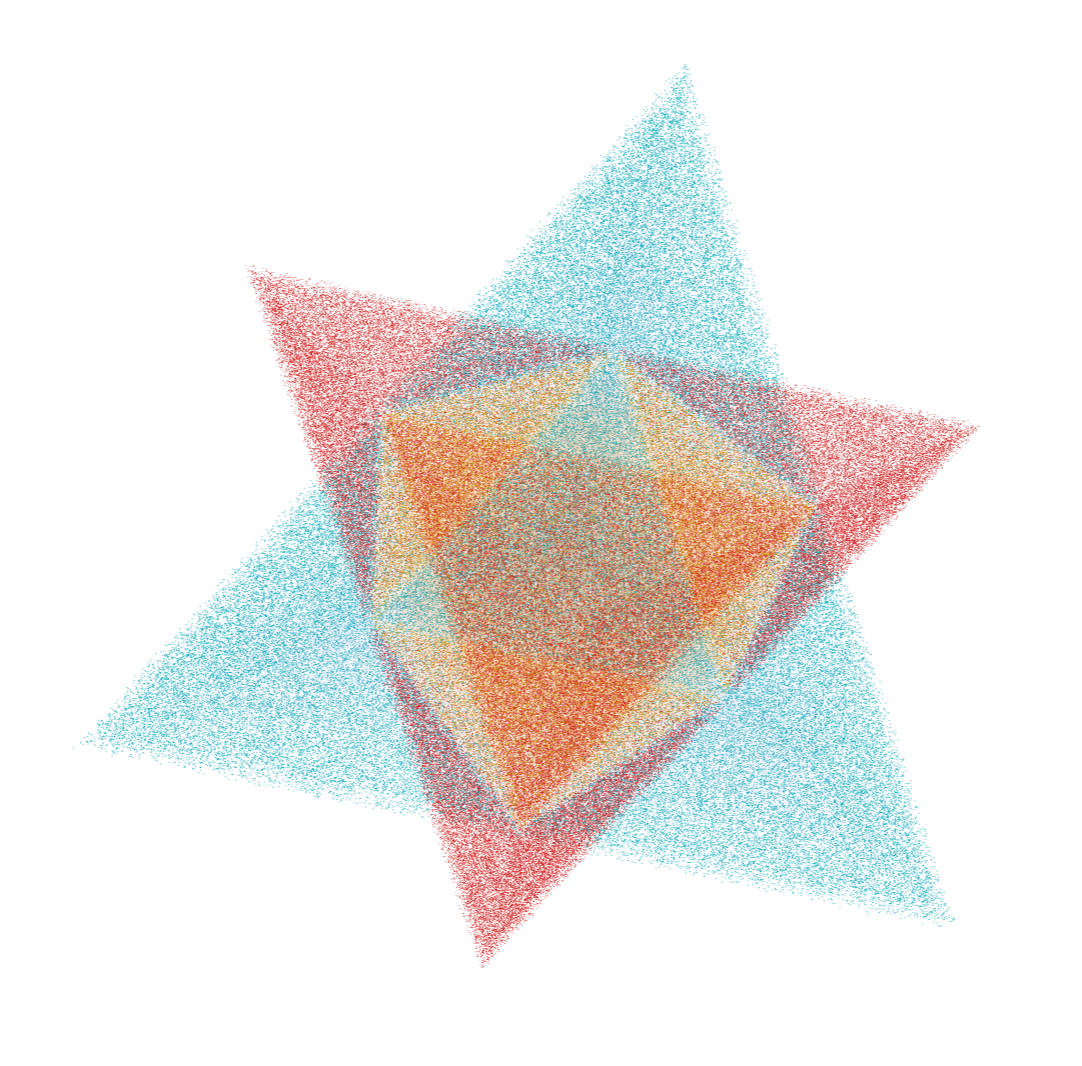
\includegraphics[width=\columnwidth]{fig1_dual_tetrahedral_field_chamber}
\caption{The dual tetrahedral field chamber. Four million points are sampled uniformly in local frame coordinates and tested against the half-space inequalities $L_i(\mathbf{p})$ defined in the text. Points that satisfy the TetA bounds are shown in cyan; those satisfying TetB in red; and those inside both (the shared octahedral Field Origin) in gold. No mesh or curve fitting is used. Each face of TetA is subdivided into three exposed corners and one inverted core where the opposing vertex penetrates, giving $4 \times 4 = 16$ geometric channels. These channels determine the gravitational coupling structure; expressed in bimetric language, they fix the interaction potential. An interactive reconstruction is provided as supplementary material.}
\label{fig1}
\end{figure}

Figure~\ref{fig1} shows the result of evaluating these half-space inequalities at four million randomly sampled points. No mesh is constructed; the geometry emerges from the boundaries alone. On each face of TetA, the penetration by TetB's opposing vertex subdivides the surface into four sub-regions: three spatial corners and one central inverted core. This $3 + 1$ subdivision, repeated across all four faces, produces $4 \times 4 = 16$ independent boundary channels.

\subsection{Face normals and binary vertices}

The four face-normal directions ($v_1$ through $v_4$) each contain three signs ($+$ or $-$). Reading $+$ as 1 and $-$ as 0 converts each normal into a 3-bit binary address. Table~\ref{tab:normals} shows the complete mapping.

\begin{table}[h]
\centering
\caption{Sign-to-binary encoding of the tetrahedral face normals.}
\label{tab:normals}
\begin{tabular}{ccccc}
\hline
Normal & Signs & Binary & Decimal & Tet \\
\hline
$v_1 = +x+y+z$ & $+\,+\,+$ & 111 & 7 & A \\
$v_2 = +x-y-z$ & $+\,-\,-$ & 100 & 4 & A \\
$v_3 = -x+y-z$ & $-\,+\,-$ & 010 & 2 & A \\
$v_4 = -x-y+z$ & $-\,-\,+$ & 001 & 1 & A \\
$-v_1$ & $-\,-\,-$ & 000 & 0 & B \\
$-v_2$ & $-\,+\,+$ & 011 & 3 & B \\
$-v_3$ & $+\,-\,+$ & 101 & 5 & B \\
$-v_4$ & $+\,+\,-$ & 110 & 6 & B \\
\hline
\end{tabular}
\end{table}

Each face of the tetrahedron points toward one specific corner of the cube. The four face normals of the primary tetrahedron point to corners 7, 4, 2, 1: the four odd-parity corners, TetA $= \{7, 4, 2, 1\}$. Negating all normals yields corners 0, 3, 5, 6: the four even-parity corners, TetB $= \{0, 3, 5, 6\}$. The stellated octahedron derived in Sections~\ref{sec:uniqueness}--\ref{sec:spacetime} from binary arithmetic and the dual tetrahedra that general relativity has used as the tetrad since 1928 are the same mathematical object.

% -- Pillar transition --

We have established what the gravitational field IS: the stellated octahedron, forced by the uniqueness theorem and identical to the tetrahedra that GR abstracts as the tetrad. But knowing what a field IS does not tell us what it DOES. A gravitational field created by a mass does not stop at an arbitrary boundary; it extends through all of space, accounting for every point. This completeness requirement is \emph{field closure}. In Einstein's general relativity, field closure is enforced by requiring the field equations to hold at every spacetime point. We now ask a different question: what does the closure requirement \emph{determine}?


% ======================================================================
\section{Coupling Constants from Geometry}
\label{sec:coupling}
% ======================================================================

\subsection{The locked parameter set}

For the field to close, the two chambers must couple. The geometry of the dual tetrahedral field chamber determines how.

TetB's penetrating vertex subdivides each face of TetA. Take any triangle and connect the midpoints of its three edges; this creates four smaller triangles, all identical in shape to the original (the medial triangle theorem). When TetB's vertex penetrates a face of TetA, it sits at the center of this four-part subdivision. Each of TetA's $K = 4$ faces acquires $4$ sub-channels, for a total of
\begin{equation}
K \times K = K^2 = 16
\end{equation}
independent coupling channels at the face-to-face boundary.

The two interlocking tetrahedra correspond, in the language of bimetric gravity~\cite{HassanRosen2012a}, to two interacting metrics with an interaction potential governed by five coefficients $\beta_0$ through $\beta_4$. These have been free parameters for over a decade. The closure geometry determines all five:
\begin{itemize}
\item $\beta_0 = \beta_4 = 1$: exchange symmetry between the two chambers fixes the boundary terms at unity.
\item $\beta_1 = \beta_3 = 0$: the two tetrahedra have opposite spatial orientations; orientation parity at the Field Origin forces all odd-order mixing to vanish.
\item $\beta_2 = K^2 = 16$: the pairwise face-to-face coupling absorbs the full channel count. The companion letter provides an independent algebraic proof: these 16 channels saturate the full dimensionality of the Clifford spacetime algebra $Cl_{1,3}$, whose $2^{D+1} = 16$ basis elements represent the complete local frame-to-frame mapping capacity~\cite{Nelson2026b}.
\end{itemize}
The complete locked set is
\begin{equation}
(\beta_0,\, \beta_1,\, \beta_2,\, \beta_3,\, \beta_4) = (1,\, 0,\, 16,\, 0,\, 1).
\end{equation}
The detailed derivation and ghost-freedom proof appear in the companion letter~\cite{Nelson2026b}. A ghost is a theoretical excitation with negative energy; if present, the vacuum is unstable and the field cannot close consistently~\cite{BoulwareDeser1972}. Ghost-freedom ensures the field CAN close; it also guarantees the existence of a Vainshtein screening mechanism~\cite{Vainshtein1972} that recovers general relativity in strong-field environments. The locked potential lies within the ghost-free Hassan--Rosen class by construction.

\subsection{The coupling polynomial}

The coupling polynomial counts the number of active geometric channels between the two tetrahedra as a function of the field's internal state. When the field is at full strength ($s = +1$), all channels are active. At the symmetric center ($s = 0$), only the even-order channels contribute. At the lower bound ($s = -1$), the count reaches its minimum. The polynomial encoding this spectrum is
\begin{equation}
f(k,\, s) = 1 + ks + k^2.
\end{equation}
At $k = K = 4$, it evaluates to three structural states:
\begin{align}
f(4,\, +1) &= 21 \quad \text{(full capacity)}, \nonumber \\
f(4,\, 0) &= 17 \quad \text{(Field Origin)}, \nonumber \\
f(4,\, -1) &= 13 \quad \text{(geometric minimum)}.
\end{align}
The closure range is $f(+1) - f(-1) = 21 - 13 = 8 = 2K = 2^D$: both twice the closure constant and the total vertex count. The field must traverse this full range to close.

The ratio of the two central values carries an algebraic signature. A continued fraction is a way of writing a number as nested divisions; for example, $17/13 = 1 + 1/(3 + 1/4)$, written $[1;\, 3,\, 4]$. The partial quotients 1, 3, 4 encode the number's internal structure. For the gravitational ratio $17/13$, these quotients are
\begin{equation}
\frac{17}{13} = [1;\, D,\, K] = [1;\, 3,\, 4],
\end{equation}
literally encoding both structural parameters from the uniqueness theorem.

\subsection{Algebraic structure of the coupling polynomial}

The coupling polynomial $f(k,s) = 1 + ks + k^2$ has a property that places it in a well-studied family. Reverse the order of its coefficients: $k^2 + sk + 1$ has the same coefficients read forward and backward. A polynomial with this symmetry is called \emph{self-reciprocal}: it satisfies $k^2 f(1/k,\,s) = f(k,\,s)$. Self-reciprocal polynomials are standard objects in algebra; their defining consequence is that if $r$ is a root, so is $1/r$.

Treating $f$ as a quadratic in $k$, the roots are $k = (-s \pm \sqrt{s^2 - 4})/2$. For every physical state $|s| \leq 1$, the discriminant $s^2 - 4$ is negative, so the roots are complex conjugates. Combined with self-reciprocity, $|r|^2 = r \cdot (1/r) = 1$: every root lies on the unit circle in the complex plane, for all $s$ in $[-1,\,+1]$.

At the two capacity endpoints, the polynomial reduces to classical cyclotomic polynomials, the polynomials whose roots are the primitive $n$th roots of unity:
\begin{align}
f(k,\,+1) &= k^2 + k + 1 = \Phi_3(k), \nonumber \\
f(k,\,-1) &= k^2 - k + 1 = \Phi_6(k).
\label{eq:cyclotomic}
\end{align}
$\Phi_3$ is the third cyclotomic polynomial; its roots are the primitive cube roots of unity. $\Phi_6$ is the sixth; its roots are the primitive sixth roots. These are textbook objects, tabulated in any algebra reference. At the capacity endpoints, the root phases are $\pi/3$ and $2\pi/3$, two adjacent vertices of the regular hexagon inscribed in the unit circle. At the Field Origin ($s = 0$), the roots sit at $\pm i$ (phase $\pi/2$), the midpoint of the arc between them. As $s$ sweeps from $-1$ to $+1$, the roots trace exactly one hexagonal sector (60 degrees) of the unit circle.

The product identity $\Phi_3(k) \cdot \Phi_6(k) = k^4 + k^2 + 1$ links the two capacity endpoints algebraically. At $k = K = 4$, this reads $21 \times 13 = 273 = 4^4 + 4^2 + 1$, confirming that the full capacity and the geometric minimum are not independent numbers but two evaluations of a single cyclotomic structure.

The coupling polynomial belongs to the cyclotomic family, the family that encodes rotational symmetry. This is a consequence of the stellated octahedron's geometry, not a design choice.


% ======================================================================
\section{The Scalar-Tensor Action}
\label{sec:action}
% ======================================================================

The coupling polynomial is a static encoding. The field must close dynamically. To extract the dynamics, we project the closure parameter onto observable quantities.

In materials science, a constitutive law relates stress to strain: it tells you how a material responds to force. In gravity, the constitutive law $\mu(x)$ plays the same role: it specifies what fraction of the expected Newtonian acceleration is actually produced at a given field strength. The dimensionless kinematic acceleration $x = |g|/a_0$ measures the local gravitational field in units of the transition acceleration scale ($a_0 \approx 1.2 \times 10^{-10}\;\text{m/s}^2$). Near a massive object ($x \gg 1$), $\mu$ approaches 1 and gravity is fully Newtonian. Far from any source ($x \ll 1$), $\mu$ drops below 1 and gravity departs from Newton's predictions. This interpolation structure was first proposed by Milgrom~\cite{Milgrom1983}; Bekenstein and Milgrom~\cite{BekensteinMilgrom1984} showed it could be derived from a scalar-tensor action.

\subsection{From topology to the constitutive law and covariant action}

The observable quantity $x$ ranges from zero to infinity. The internal state parameter $s$ ranges from $-1$ to $+1$. The unique smooth map connecting these two ranges while fixing the transition point ($x = 1$, $s = 0$) at the center is the Mobius transformation
\begin{equation}
s(x) = \frac{x - 1}{x + 1}.
\end{equation}
Composing $f(K,\, s(x))$ gives the continuous topological capacity:
\begin{equation}
f(x) = \frac{21x + 13}{x + 1},
\end{equation}
which interpolates smoothly between the geometric minimum ($f = 13$ at $x = 0$) and the full capacity ($f \to 21$ as $x \to \infty$).

Normalizing $f(x)$ to the range $[0, 1]$ asks: what fraction of the total capacity range is being used? The formula is $\mu = (f - 13)/(21 - 13) = (f - 13)/8$. Substituting:
\begin{align}
\mu(x) &= \frac{1}{8}\left(\frac{21x + 13}{x + 1} - 13\right) \nonumber \\[4pt]
&= \frac{1}{8} \cdot \frac{21x + 13 - 13x - 13}{x + 1} \nonumber \\[4pt]
&= \frac{1}{8} \cdot \frac{8x}{x + 1} = \frac{x}{x + 1}.
\label{eq:mu}
\end{align}
The factor of 8 cancels perfectly. This cancellation is not a coincidence; it is the vertex count $2^D$ eliminating itself from the constitutive law, leaving a function determined entirely by the topology.

The constitutive law tells us the local field response. A complete gravitational theory also requires an action, a Lagrangian from which the field equations follow variationally. Integrating the constitutive law via $\mu(\sqrt{y}) = dF/dy$ (with $y = |\nabla\Phi|^2/a_0^2$) yields the kinetic functional
\begin{equation}
F(y) = y - 2\sqrt{y} + 2\ln\!\left(1 + \sqrt{y}\right),
\end{equation}
with the boundary condition $F(0) = 0$ fixing the integration constant. The complete covariant scalar-tensor action is then
\begin{equation}
S = \int d^4x\,\sqrt{-g}\left[\frac{R}{16\pi G} - \frac{a_0^2}{8\pi G}\,F\!\left(\frac{|\nabla\Phi|^2}{a_0^2}\right) + \mathcal{L}_\text{m}\right].
\label{eq:action}
\end{equation}
The three coupling scales in this action are $16\pi G$, $8\pi G$, and $1/4$, with numerical prefactors 16, 8, 4. These are $K^2$, $2K$, $K$: the face-channel count, the vertex count, and the face count. Each is half the previous. The hierarchy of gravitational coupling strengths is the counting sequence of the stellated octahedron.

Every coefficient in the action is fixed. The constitutive law governs local response; the action governs global dynamics. Neither is fitted; both follow from the stellated octahedron's closure capacity.


% ======================================================================
\section{Structural Completeness}
\label{sec:completeness}
% ======================================================================

Claiming zero free parameters requires proof. Table~\ref{tab:constants} exhibits every numerical constant in the theory as a function of $K = 4$ and $D = 3$.

\begin{table}[h]
\centering
\caption{Every constant in the theory reduces to $K$ and $D$.}
\label{tab:constants}
\begin{tabular}{ccl}
\hline
Value & Expression & Physical meaning \\
\hline
4 & $K$ & Faces per tetrahedron \\
8 & $2^D$ & Vertices of the cube \\
12 & $KD$ & Edges of the stellated octahedron \\
13 & $KD + 1$ & Edges + Field Origin \\
16 & $K^2$ & Coupling channels \\
17 & $K^2 + 1$ & Capacity at Field Origin \\
21 & $K^2 + K + 1$ & Full capacity \\
64 & $K^D$ & Vertex-pair state space \\
\hline
\end{tabular}
\end{table}

The three gravitational coupling scales (16, 8, 4) form the geometric halving sequence $K^2$, $2K$, $K$: face channels, vertices, faces. The continued fraction $17/13 = [1;\, D,\, K]$ encodes both structural parameters as partial quotients. The theory has exactly two structural parameters, both fixed by the uniqueness theorem. Closure is total: no constant is imported from outside the stellated octahedron.


% ======================================================================
\section{N-Metric Screening Family}
\label{sec:nmetric}
% ======================================================================

The constitutive law $\mu(x) = x/(x+1)$ derived in Section~\ref{sec:action} corresponds to a single dynamical metric sector ($N = 1$). The framework admits a natural generalization: when $N$ metric sectors participate in the closure, the screening equation becomes
\begin{equation}
x(1 - \mu)^N = \mu.
\end{equation}
At $N = 1$, this recovers $\mu(x) = x/(x+1)$. At $N = 2$, both metrics in the bimetric theory are dynamical, yielding a distinct constitutive law.

At the transition scale $x = 1$, the $N = 1$ theory gives $\mu(1) = 1/2$. For $N = 2$, the screening equation becomes $\mu^2 - 3\mu + 1 = 0$, a quadratic whose physical root is
\begin{equation}
\mu(1) = \frac{3 - \sqrt{5}}{2} = \frac{1}{\varphi^2} \approx 0.382,
\end{equation}
where $\varphi = (1 + \sqrt{5})/2$ is the golden ratio. The appearance of $\varphi$ is not incidental: it is the algebraic consequence of requiring both metric sectors to close simultaneously.

Away from the transition point, the $N = 2$ screening equation can be solved in closed form. The full bimetric constitutive law is
\begin{equation}
\mu_2(x) = \frac{\sqrt{1 + 4x} - 1}{\sqrt{1 + 4x} + 1},
\label{eq:mu2}
\end{equation}
which satisfies $x(1 - \mu_2)^2 = \mu_2$ identically. At $x = 1$, this reduces to $({\sqrt{5} - 1})/({\sqrt{5} + 1}) = 1/\varphi^2$, recovering the golden ratio root above.

Both constitutive laws share the same asymptotic structure. In the strong-field regime ($x \gg 1$), both approach $\mu \to 1$: gravity is unmodified. In the weak-field regime ($x \ll 1$), both approach $\mu \to x$: the linear scaling characteristic of the deep-field limit. The two laws are indistinguishable in both extremes and separate only near $x \approx 1$, where the field is changing character. The $N$-metric family thus forms a discrete algebraic hierarchy indexed by closure depth, each member fully determined by the topology with zero free parameters.


% ======================================================================
\section{Algebraic Isomorphism: Pi and the Stellated Octahedron}
\label{sec:pi}
% ======================================================================

The topology defines the state space. The closure requirement demands that the field visit the complete state space without omission. The base-8 expansion of pi realizes this traversal: its digit sequence walks the eight vertices of the stellated octahedron via cumulative sum mod 8, visiting every vertex with uniform frequency.

Just as numbers are normally written in base 10 (digits 0--9), they can be written in base 8 (digits 0--7). The stellated octahedron has 8 vertices, labeled 0 through 7. Pi in base 8 ($3.11037\ldots$) produces a sequence of octal digits, each naming one of the eight vertices.

Starting at vertex 0, the first octal digit of pi after the decimal point is 1: move to vertex $(0 + 1) \bmod 8 = 1$. The next digit is 1: move to $(1 + 1) \bmod 8 = 2$. The next is 0: stay at $(2 + 0) \bmod 8 = 2$. The next is 3: move to $(2 + 3) \bmod 8 = 5$. Continuing this cumulative-sum-mod-8 walk, every vertex is visited within finitely many steps. Over many digits, each of the 8 vertices is visited with approximately equal frequency; no vertex is favored or avoided.

Under this traversal, the time face $\{1, 2, 4\}$ completes first (at step 5). Temporal structure is established before full spatial closure, consistent with the $(3+1)$ face classification of Section~\ref{sec:spacetime}.

\subsection{The BBP bridge}

In 1997, Bailey, Borwein, and Plouffe~\cite{BBP1997} discovered a formula that computes any individual hexadecimal (base-16) digit of pi without first computing all the preceding digits. This formula was a result in pure number theory, with no connection to geometry or gravity. Its internal structural constants are:
\begin{itemize}
\item Period: $8 = 2^D$ (the vertex count).
\item Active terms per period: $4 = K$ (the face count).
\item Geometric series base: $16 = K^2 = 2^K$ (the channel count).
\item Denominator coefficients: $\{+4, -2, -1, -1\}$, which sum to zero (Field Origin symmetry) and have magnitudes $\{4, 2, 1\}$, the binary place values that define the 3-bit coordinate encoding.
\end{itemize}
The three structural constants of the BBP formula (8, 4, 16) are exactly the vertex count, face count, and channel count of the stellated octahedron. The two frames (base-8 traversal and base-16 extraction) realign every $\text{lcm}(3, 4) = 12 = KD$ binary digits: the edge count of the stellated octahedron.

That these structural constants (period 8, base 16, four active terms) are identically the vertex count, channel count, and face count of the stellated octahedron demonstrates that pi natively possesses the $O_h$ symmetric structure of the $K = 4$, $D = 3$ dual-tetrahedral topology. This is an algebraic isomorphism, not a numerical coincidence.


% ======================================================================
\section{Discussion}
\label{sec:discussion}
% ======================================================================

\subsection{Summary and outlook}

The derivation chain from combinatorial identity to covariant action is:
\begin{gather*}
d\!=\!3 \;\to\; \text{stellated oct.} \;\to\; (3\!+\!1) \;\to\; \text{tetrad} \\
\to\; \{\beta_n\} \;\to\; \Phi_3/\Phi_6 \;\to\; \mu(x) \;\to\; S_\text{SST}
\end{gather*}
Each link is a theorem or a necessary consequence:
\begin{enumerate}
\item The uniqueness theorem fixes $d = 3$ (Section~\ref{sec:uniqueness}).
\item Binary parity in $d = 3$ produces the stellated octahedron (Section~\ref{sec:topology}).
\item Face classification yields the $(3+1)$ spacetime decomposition (Section~\ref{sec:spacetime}).
\item The face normals recover the tetrahedron that GR abstracts as the tetrad (Section~\ref{sec:tetrad}).
\item Face geometry locks all five bimetric coefficients $\{\beta_n\} = \{1, 0, 16, 0, 1\}$ (Section~\ref{sec:coupling}).
\item The coupling polynomial is cyclotomic ($\Phi_3$ and $\Phi_6$), with roots on the unit circle (Section~\ref{sec:coupling}).
\item Capacity normalization yields $\mu(x) = x/(x+1)$ (Section~\ref{sec:action}).
\item Integration gives the kinetic functional and the covariant action~(\ref{eq:action}) (Section~\ref{sec:action}).
\item The N-metric screening family forms a discrete algebraic hierarchy indexed by closure depth (Section~\ref{sec:nmetric}).
\end{enumerate}
The reader can verify each step independently using the companion script \texttt{run\_all\_validations.py}, which tests all nine links in sequence.

The tetrahedron recovered at step 4 is the same geometric object that appears across simplicial gravity, tetrad gravity, loop quantum gravity, and bimetric gravity (Table~\ref{tab:heritage}). GFD is the first formalism in which both the topology and the closure condition are derived rather than supplied as inputs. The algebraic isomorphism between pi's base-8 structure and the stellated octahedron (Section~\ref{sec:pi}) provides independent confirmation that the $O_h$ symmetric topology is a native feature of the mathematical constants themselves.

Two open questions remain: the extension to quantum gravity (where the closure frequency ${\sim}10^{20}$~Hz becomes relevant); and the explicit closed-form EFT matching from the locked Galileon hierarchy to the IR constitutive law, framed as a checkable matching problem in the companion letter~\cite{Nelson2026b}.

% ======================================================================
\section*{Data and Reproducibility}
% ======================================================================

All algebraic derivations are self-contained and reproducible from the equations presented. The foundational framework, including the full coupling derivation and ghost-freedom proof, is provided in the companion letter~\cite{Nelson2026b}. The point-cloud visualization in Figure~\ref{fig1} was generated by evaluating the four tetrahedral half-space inequalities at four million uniformly sampled points; the rendering code is provided as supplementary material. An interactive three-dimensional reconstruction of the dual tetrahedral field chamber (\texttt{fig1\_dual\_tetrahedral\_field\_chamber.html}) is also included, allowing the reader to rotate, zoom, and inspect the geometry directly. A companion validation script (\texttt{run\_all\_validations.py}) independently verifies every claim in this letter through 45 tests across 19 sections: topology (Sections~\ref{sec:uniqueness}--\ref{sec:tetrad}), field closure (Sections~\ref{sec:coupling}--\ref{sec:pi}), cyclotomic structure, N-metric algebra, and the complete derivation chain. All three files are included as supplementary material.


% ======================================================================
\section*{Acknowledgements}
% ======================================================================

The author acknowledges the ghost-free bimetric framework of S.~F.~Hassan and R.~A.~Rosen, the tetrad gravity formalism developed by Cartan, Einstein, Weyl, and Ashtekar, and the BBP digit-extraction formula of Bailey, Borwein, and Plouffe.


% ======================================================================
\begin{thebibliography}{99}

\bibitem{Nelson2026b}
S.~Nelson,
``Gravity Field Dynamics and Bimetric Gravity: Dual Tetrahedral Field Chambers as the Key to the General Parameters,''
submitted to \textit{Class. Quantum Grav.} (2026).

\bibitem{HassanRosen2012a}
S.~F.~Hassan and R.~A.~Rosen,
``Bimetric gravity from ghost-free massive gravity,''
\textit{J. High Energy Phys.} \textbf{2012}(02), 126 (2012).

\bibitem{Einstein1928}
A.~Einstein,
``Riemann-Geometrie mit Aufrechterhaltung des Begriffes des Fernparallelismus,''
\textit{Sitzungsber. Preuss. Akad. Wiss.} (1928), 217.

\bibitem{Weyl1929}
H.~Weyl,
``Elektron und Gravitation. I,''
\textit{Z. Phys.} \textbf{56}, 330 (1929).

\bibitem{Milgrom1983}
M.~Milgrom,
``A modification of the Newtonian dynamics as a possible alternative to the hidden mass hypothesis,''
\textit{Astrophys. J.} \textbf{270}, 365 (1983).

\bibitem{BekensteinMilgrom1984}
J.~Bekenstein and M.~Milgrom,
``Does the missing mass problem signal the breakdown of Newtonian gravity?''
\textit{Astrophys. J.} \textbf{286}, 7 (1984).

\bibitem{BBP1997}
D.~Bailey, P.~Borwein, and S.~Plouffe,
``On the rapid computation of various polylogarithmic constants,''
\textit{Math. Comp.} \textbf{66}, 903 (1997).

\bibitem{Vainshtein1972}
A.~I.~Vainshtein,
``To the problem of nonvanishing gravitation mass,''
\textit{Phys. Lett. B} \textbf{39}, 393 (1972).

\bibitem{BoulwareDeser1972}
D.~G.~Boulware and S.~Deser,
``Can gravitation have a finite range?''
\textit{Phys. Rev. D} \textbf{6}, 3368 (1972).

\bibitem{Regge1961}
T.~Regge,
``General relativity without coordinates,''
\textit{Nuovo Cimento} \textbf{19}, 558 (1961).

\bibitem{RovelliSmolin1995}
C.~Rovelli and L.~Smolin,
``Spin networks and quantum gravity,''
\textit{Phys. Rev. D} \textbf{52}, 5743 (1995).

\bibitem{Israel1966}
W.~Israel,
``Singular hypersurfaces and thin shells in general relativity,''
\textit{Nuovo Cimento B} \textbf{44}, 1 (1966).

\end{thebibliography}

\end{document}
